\documentclass[tikz,border=10pt]{standalone}
\usepackage{pgfplots}
\usepgfplotslibrary{fillbetween}
\pgfplotsset{compat=1.18}
\begin{document}
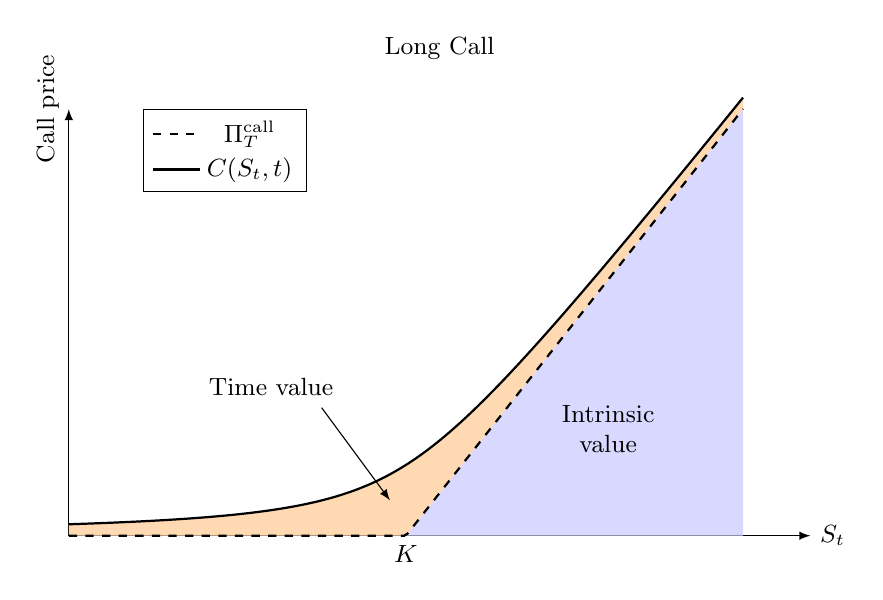
\begin{tikzpicture}[font=\small]
  \pgfmathsetmacro{\K}{1}        % strike price
  \pgfmathsetmacro{\RefPt}{1.5}  % reference point used to size the hyperbola's gap
  \pgfmathsetmacro{\Gap}{0.05}   % desired vertical gap (time value) AT the reference point
  \pgfmathsetmacro{\C}{\Gap*(\Gap+abs(\RefPt-\K))}
  \begin{axis}[
      width=11cm, height=7cm,
      axis x line=bottom,
      axis y line=left,
      axis line style={-latex},
      xmin=0, xmax=2.2,
      ymin=0, ymax=1,
      xtick=\empty, ytick=\empty,
      domain=0:2,
      samples=200,
      clip=false,
      xlabel={$S_t$},
      xlabel style={at={(axis description cs:1,0)}, anchor=west},
      ylabel={Call price},
      ylabel style={at={(axis description cs:0,1)}, anchor=south},
      title style={
          at={(axis description cs:0.5,1)},
          yshift=0.3cm,
          anchor=south,
        },
      title={Long Call},
      legend style={at={(axis description cs:0.1,1)}, anchor=north west},
    ]

    %  invisible named paths (needed by fillbetween) 
    \addplot[name path=payoff, draw=none, forget plot] {max(x-\K,0)};
    \addplot[name path=priceline, draw=none, forget plot] {(  (x-\K) + sqrt((x-\K)^2 + 4*\C)  )/2};
    \addplot[name path=xaxis, draw=none, forget plot] {0};

    %  shaded areas 
    \addplot[blue!15, forget plot] fill between[of=payoff and xaxis];      % intrinsic value
    \addplot[orange!30, forget plot] fill between[of=priceline and payoff]; % time value

    %  redraw the visible curves on top of the fills 
    \addplot[dashed, thick] {max(x-\K,0)}; \addlegendentry{$\Pi_T^\mathrm{call}$}
    \addplot[solid, thick] {(  (x-\K) + sqrt((x-\K)^2 + 4*\C)  )/2}; \addlegendentry{$C(S_t, t)$}

    \node[below] at (axis cs:\K,0) {$K$};

    %  region labels 
    \node[align=center] at (axis cs:1.6,0.25) {Intrinsic\\value};

    \node[align=center] at (axis cs:0.6,0.35) {Time value};
    \draw[-latex, shorten >=1.5pt] (axis cs:0.75,0.30) -- (axis cs:0.96,0.075);

  \end{axis}
\end{tikzpicture}
\end{document}